\chapter{Evaluation}
\label{chapter:evaluation}

An evaluation of the intersection unit transfer-relation model in Section~\ref{sec:c_c_isect_modeling} is provided in this section.

\section{Intersection unit transfer-relation model}

\subsection{Methodology}

The intersection unit transfer relation model was trained on a dataset generated by a cycle accurate simulator. The simulator was used to create train and test datasets. Dataloaders with batch size 1000 were created. The loss function was MSE of the difference between the predicated and actual estimates of match rate associated with the intersection unit. The model was fitted to a single batch from the training dataset. The percentage error in predicting match rate was evaluated against the test dataset.

It was observed empirically that it was challenging to fit a model to the full range of sparsities from 0\% to 100\%; the model was only trained and tested over the range of sparsities from 30\% to 70\%.

\subsection{Result}

\begin{figure}[ht]
    \centering
    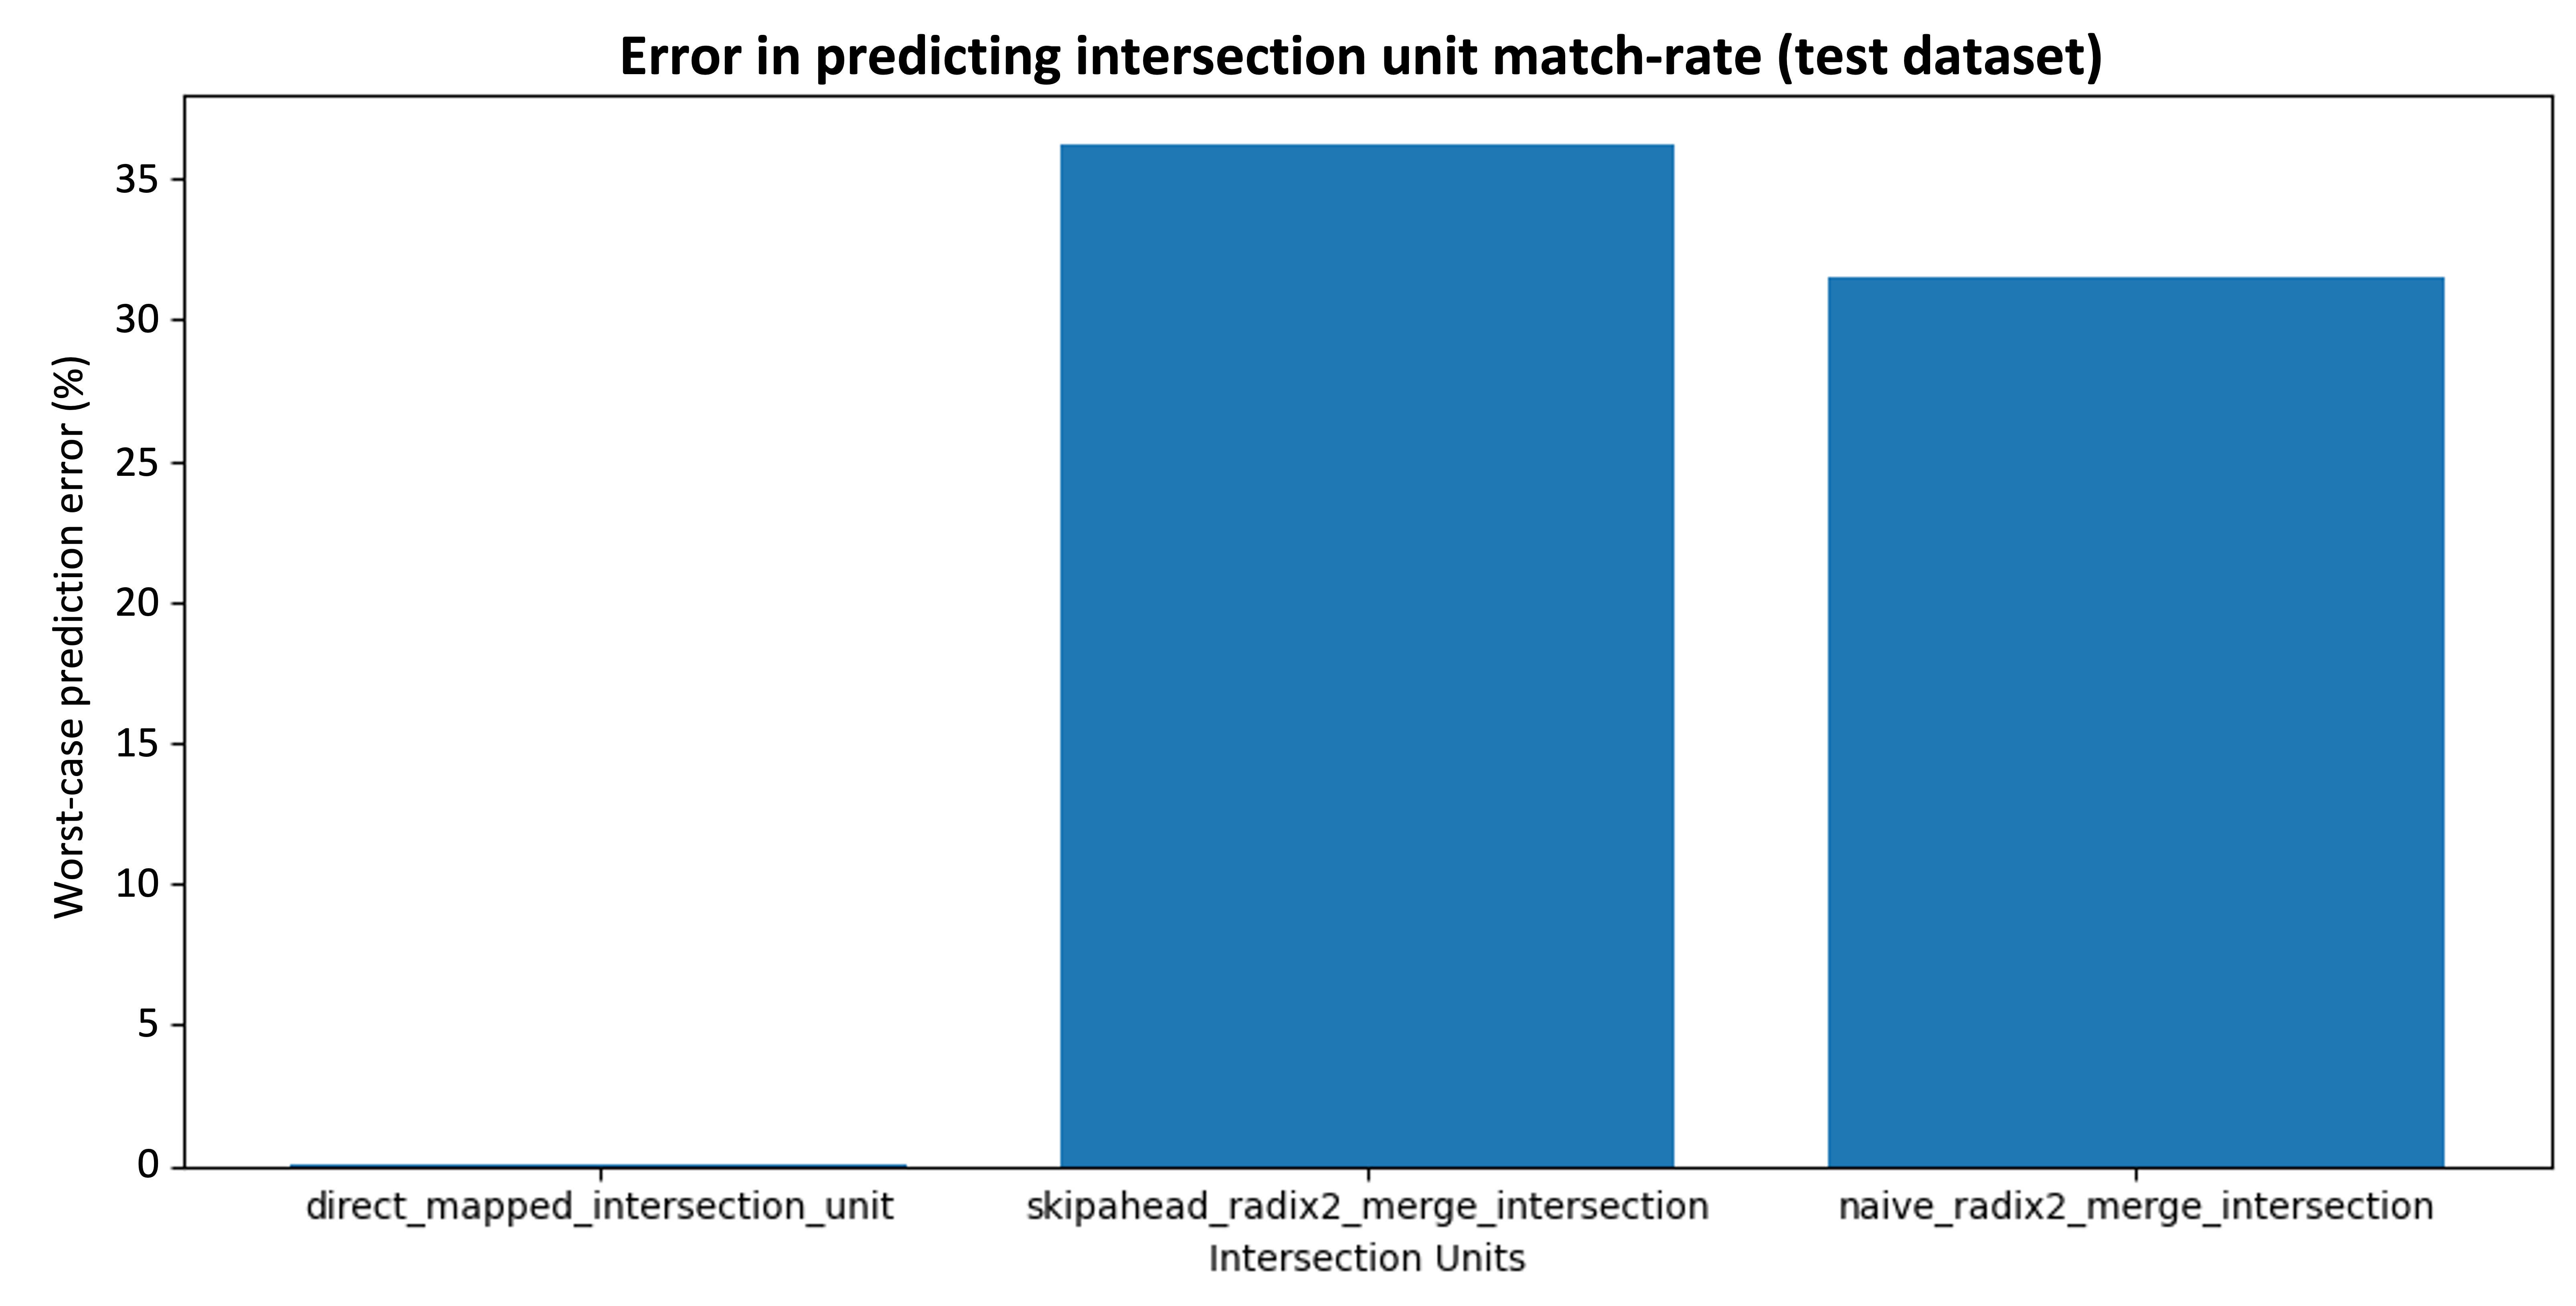
\includegraphics[width=0.95\textwidth]{figures/isect_test_error.png}
    \caption{Intersection unit analytical model validation against three intersect unit types (\textit{direct-mapped}, \textit{naive two-finger intersection}, and \textit{skip-ahead intersection}).}
    \label{fig:isect_test_error}
\end{figure}

Figure~\ref{fig:isect_test_error} shows the percentage error in predicting match rate for each type of intersection unit. Note that the percentage error is less that 40\% for all for all intersection unit types, which is considered sufficient for modeling in this work.